\problem{}
Consider an $n \times n$ grid containing $n$ rows and $n$ columns of vertices.  Each vertex $(i, j)$ has edges to four neighbors $(i-1, j)$, $(i+1, j)$, $(i, j-1)$, $(i, j+1)$, except for the boundary vertices, which have edges to two or three neighbors.  Each vertex and edge also has a positive integer capacity.  We are given $m $ start vertices, and for each vertex we want to find a path which connects the vertex to an arbitrary vertex on the grid's boundary.  Furthermore, we need to ensure that the number of paths which pass through each vertex or edge does not exceed its capacity.  Give an algorithm to determine whether this is possible. \\

\noindent \emph{Hint:}  First transform the graph to convert the vertex capacities to edge capacities.  

\solution{}
\begin{figure}[htbp]
    \centering
    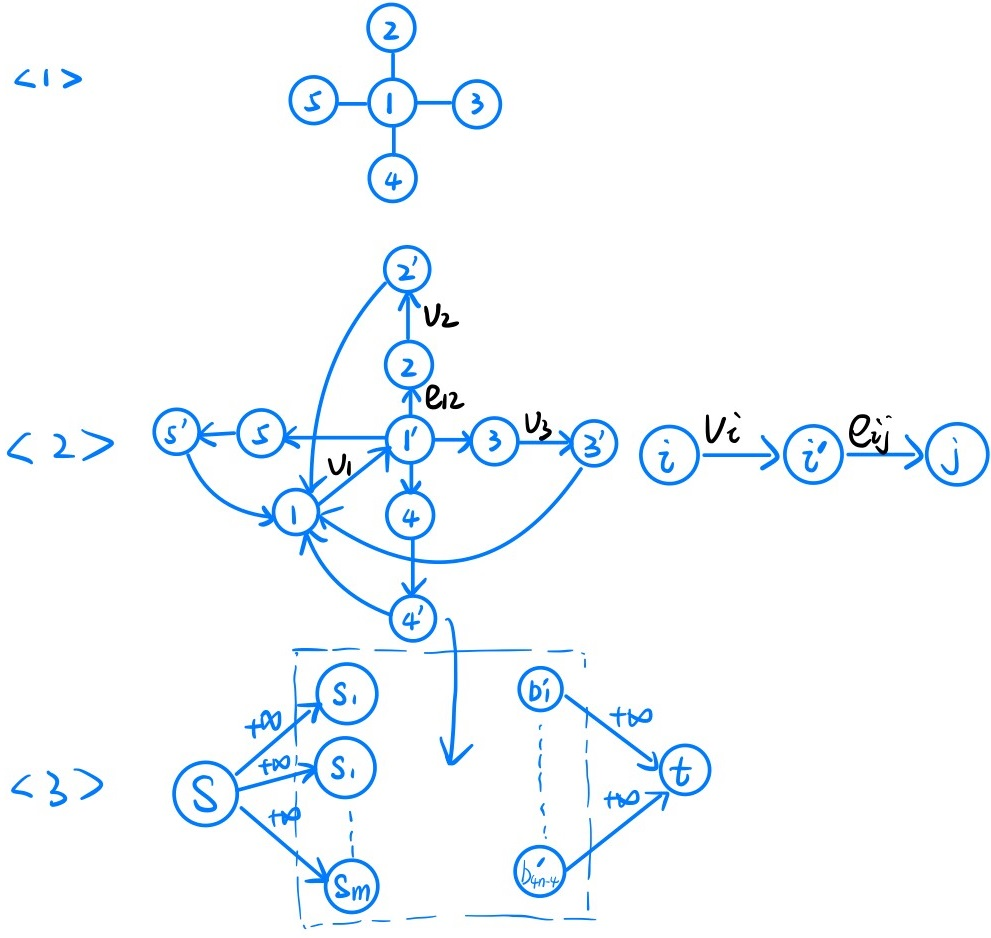
\includegraphics[width=0.9\linewidth]{../fig/p4.png}
    \caption{Way to contrust the graph}
    \label{fig:p4}
\end{figure}

We can construct the graph as the Figure \ref{fig:p4} shows.

The details are as follows:

Each node $u$ is seperated into $2$ new node, a in node $u$ and an out node $u'$.

Supoose each node is given a number to represent a grid. The neibor nodes $(i,j)$'s edge's capacity is $c_{i,j}$, the node $i$'s capacity is $v_i$.

The start vertices are $s_1,s_2,\cdots,s_m$, the boundary nodes are $b_1,\cdots,b_{4n-4}$.

1. To make sure the limitations of vertex and edge's capacity, we need to split each node $i$ into $i$ and $i'$, and we let $i$ to recieve connections from other nodes, $i'$ to give out connections to other nodes.

As shown in Figure \ref{fig:p4}'s <2> part, we set edge from $i$ to $i'$ with capacity $v_i$.

If node $i$ and node $j$ have connections such as in <1>, then we set up edge from $i'$ to $j$ with capacity $e_{i,j}$, and similarly, an edge from $j'$ to $i$ with capacity $e_{i,j}$.

2. We set up edges from $s$ to $s_i, i=1,2,\cdots,m$ with capacity $+\infty$.

3. We set up edges from the boundary nodes $b_1',\cdots,b_{4n-4}'$ to $t$ with capacities $+\infty$.

Then the graph is contrusted.

Let $C=\max\left\{\max\{c_{i,j}\},D=\max\{v_i\}\right\}$\\
From our construction methods, we can find the sink node $s$ is only sending flow to $s_1,\cdots,s_m$, 
and the boundary nodes $b_j'$ recieves flow only from $b_j$.\\
So we can just set the $+\infty$ to be $C$.\\

With above construction, we can use the Ford-Fulkerson algorithm to find the maximum flow of the constructed graph. 

If the maximum flow is the number of paths the graph can have which suits the requirements.\\
The time complexity is $O(n^4\log C)$.\\
Since each grid is seperate into two nodes, but the nodes' edges are constant, so the number of the edges in the constructed graph is $O(n^2)$.\\

\newpage